%* 
%* ------------------------------------------------------------------
%* LocoPullManual.tex - LocoPull Manual
%* Created by Robert Heller on Mon Mar 22 15:23:08 2010
%* ------------------------------------------------------------------
%* Modification History: $Log$
%* Modification History: Revision 1.1  2002/07/28 14:03:50  heller
%* Modification History: Add it copyright notice headers
%* Modification History:
%* ------------------------------------------------------------------
%* Contents:
%* ------------------------------------------------------------------
%*  
%*     Model RR System, Version 2
%*     Copyright (C) 1994,1995,2002-2005  Robert Heller D/B/A Deepwoods Software
%* 			51 Locke Hill Road
%* 			Wendell, MA 01379-9728
%* 
%*     This program is free software; you can redistribute it and/or modify
%*     it under the terms of the GNU General Public License as published by
%*     the Free Software Foundation; either version 2 of the License, or
%*     (at your option) any later version.
%* 
%*     This program is distributed in the hope that it will be useful,
%*     but WITHOUT ANY WARRANTY; without even the implied warranty of
%*     MERCHANTABILITY or FITNESS FOR A PARTICULAR PURPOSE.  See the
%*     GNU General Public License for more details.
%* 
%*     You should have received a copy of the GNU General Public License
%*     along with this program; if not, write to the Free Software
%*     Foundation, Inc., 675 Mass Ave, Cambridge, MA 02139, USA.
%* 
%*  
%* 

\chapter{LocoPull Program Reference}
\label{chpt:locopull:Reference}
\typeout{$Id$}

\section{Basis and Mathematics}
This program is based on the information posted by Mark U. on the Yahoo
XTrkCad list\footnote{At the URL
\url{http://groups.yahoo.com/group/XTrkCad/message/4983}.} and the
information supplied by rtroop on the TrainBoard forum\footnote{Post
\#9 at the URL
\url{http://www.trainboard.com/grapevine/showthread.php?t=114497}.}.
This is a standalone program that incorporates the formulas presented in
Mark U's spreadsheet and explained in rtroop's message.  The formulas
are as follows:

\begin{eqnarray}
E_{unit} &=& W_{unit}{A} \label{eq:locopull:teperunit} \\
E  &=& E_{unit}{N} \label{eq:locopull:tenet} \\
R_{ave}  &=& W_{ave}{F} \label{eq:locopull:aveRR} \\
C_{0~Grade} &=& \Biggl\lfloor \frac{E}{R_{ave}} \Biggr\rfloor \label{eq:locopull:zgrade} \\
R_{grade}    &=& W_{ave}{G} \label{eq:locopull:rraddedgrade} \\
R_{net~at~grade} &=& R_{ave} + R_{grade} \label{eq:locopull:rratgrade} \\
R_{unit~at~grade} &=& W_{unit}{G} \label{eq:locopull:rrunitgrade} \\
D &=& \frac{5730}{\frac{rS}{12}} \label{eq:locopull:degreecurve} \\
C_{grade~and~curve} &=& \Biggl\lfloor 
     \frac{ {E} - {N} {W_{unit}} ( G + F + D ) }
          { {R_{ave}} + {W_{ave}} ( G + {F_{per~degree}}
							{D} ) } 
	\Biggr\rfloor \label{eq:locopull:capatgradecurve}
\end{eqnarray}



\begin{tabular}{rrp{3in}}
Where:&&\\
&$W_{unit}$ &is the weight of each locomotive in ounces. \\
&$A$ &is the adhesion factor generally 25\%. \\
&$E_{unit}$&is the tractive effort per unit in ounces. \\
&$E$&is the net tractive effort in ounces. \\
&$N$&is the number of units. \\
&$F$ &is the resistance factor of each car, typically 4\% for N
scale cars.\\
&$W_{ave}$&is the average weight per car, typically 1 ounce for N scale cars.\\
&$R_{ave}$&is the average rolling resistance of each car.\\
&$C_{0~Grade}$&is the capacity of the train on level, straight
track.\\
&$G$&is the percent of grade.\\
&$R_{grade}$&is the added rolling resistance of each car due to
grade.\\
&$R_{net~at~grade}$&is the net rolling resistance of each car at
grade.\\
&$r$ &is the track radius in inches.\\
&$S$&is the scale factor (160 for N scale, 87 for H0 scale, etc.).\\
&$D$& is the degree of curvature.\\
&$F_{per~degree}$&is the resistance factor per degree of curvature,
typically .04\%.\\
&$C_{grade~and~curve}$&is the capacity of the train on at grade on a
curve.\\
\end{tabular}

\section{The GUI}
\begin{figure}[hbpt]
\begin{centering}
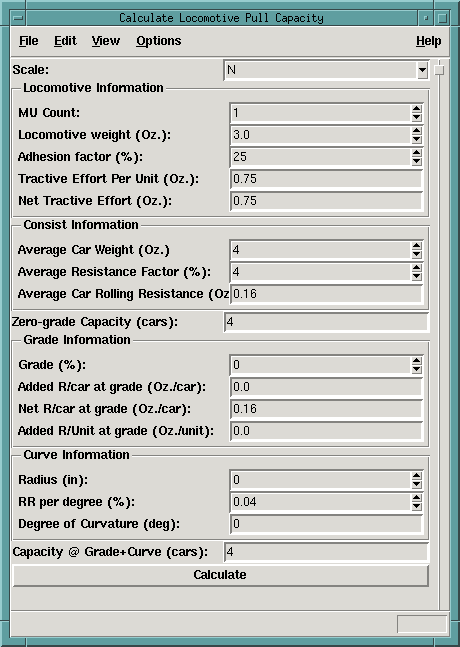
\includegraphics[width=5in]{LocoPullMain.png}
\caption{The main GUI screen of the LocoPull program}
\label{fig:locopull:main}
\end{centering}
\end{figure}
The main GUI screen of the LocoPull program is shown in
Figure~\ref{fig:locopull:main}. The GUI is broken down into sections: 
\begin{itemize}
\item The Scale section.  The scale is selected here.
\item The Locomotive Information section.  Information about the
locomotives is entered here.  The number of locomotives, how much they
weigh each, and their adhesion factor. The tractive effort for each unit
and the net tractive effort are computed and displayed here. It is
assumed that all of the powered engines are the same, typically the same
make and model, with the same weight and same adhesion factor.
\item The Consist Information. Information about the cars, including
their average weight and their average resistance factor are entered and
the rolling rolling resistance is computed and displayed.
\item The Zero-grade Capacity section.  The maximum number of cars that
can be pulled on a straight track on a level grade is computed and
displayed here.
\item The Grade Information section. The percent of grade is entered and
the added rolling resistance per car at grade, the net rolling
resistance, and the added resistance per unit are computed and displayed
here. 
\item The Curve Information section. The radius of the curve in inches
and the rolling resistance per degree of curve are entered and the
degree of curvature is computed and displayed.
\item The Capacity at Grade and Curve section.  This is the maximum
number of cars that can be pulled at the grade and curve specified.
\item Calculate button. This button performs the calculation and updates
all of the displayed values.
\end{itemize}

\subsection{The Scale}
The scale selection simply select the scale and is used to compute the
degree of curvature.

\subsection{Locomotive Information}
This section of the GUI gathers information about the locomotives
pulling the train.  It is assumed that all of the locomotives have the
same tractive effort, that is they are the same weight and have the same
adhesion factor.  This would generally be the case if the locomotives
were the make and model.  Three inputs are gathered in this section: the
number of locomotives, the weight of each locomotive, and the adhesion
factor of the locomotives.  Two intermediate outputs are displayed here:
the tractive effort of each locomotive and the net tractive effort of
all of the locomotives together.

\subsection{Consist Information}
This section gathers two inputs and displays one intermediate result. 
The two inputs are the average weight of the cars and the average
rolling resistance factor.  The intermediate result is the average car
rolling resistance.

\subsection{Zero-grade capacity}
This is simply the net tractive effort divided by the average car
rolling resistance.  The floor of the result is displayed as a whole
number (since pulling a fraction of a car is not meaningful).

\subsection{Grade information}
One input is gathered and three intermediate results are displayed.  The
input is the percent of grade and the intermediate results displayed are
the added rolling resistance at grade of each car, the net rolling
resistance per car, and the added rolling resistance of each locomotive
at grade.

\subsection{Curve information}
This section gathers two inputs and displays one intermediate result.
The added inputs are the curve radius and the rolling resistance per
degree of curvature and the intermediate result is the degree of
curvature. 

\subsection{Capacity and Grade plus Curve}
This is just the tractive effort less the tractive effort needed to
pull the locomotives themselves divided by the combined rolling
resistance of the average car: base rolling resistance plus the added
rolling resistance due to grade, plus the added rolling resistance due
to the curvature.  The floor of the result is displayed as a whole
number (since pulling a fraction of a car is not meaningful).



